% ─────────────────────────────────────────────────────────────────────────────
% scordatura — slide deck (house style). Compile: lualatex scordatura_slides.tex (twice)
% ─────────────────────────────────────────────────────────────────────────────
\documentclass[aspectratio=169,11pt]{beamer}
\usetheme{metropolis}

\usepackage{amsmath,amssymb}
\usepackage{booktabs}
\usepackage{pifont}
\usepackage{tikz}
\usetikzlibrary{
  arrows.meta,positioning,calc,
  decorations.pathreplacing,decorations.markings,
  shapes.geometric,shapes.misc,
  backgrounds,fit,patterns
}
\usepackage{fontspec}

% ══ PALETTE ═══════════════════════════════════════════════════════════════════
\definecolor{mainblue}{HTML}{3B82F6}
\definecolor{maindark}{HTML}{1E3A5F}
\definecolor{fwdgreen}{HTML}{22C55E}
\definecolor{fwddark}{HTML}{14532D}
\definecolor{arrowyellow}{HTML}{EAB308}
\definecolor{grayout}{HTML}{9CA3AF}
\definecolor{streamgray}{HTML}{64748B}
\definecolor{gateorange}{HTML}{F97316}
\definecolor{gatedark}{HTML}{7C2D12}
\definecolor{warmred}{HTML}{EF4444}
\definecolor{softpurple}{HTML}{8B5CF6}
\definecolor{slate50}{HTML}{F8FAFC}
\definecolor{slate100}{HTML}{F1F5F9}
\definecolor{slate200}{HTML}{E2E8F0}
\definecolor{slate700}{HTML}{334155}
\definecolor{slate800}{HTML}{1E293B}

\definecolor{learned}{HTML}{F97316}
\definecolor{frontier}{HTML}{EA580C}
\definecolor{unlearned}{HTML}{E2E8F0}

\colorlet{lvlc0}{mainblue!20}
\colorlet{lvlc1}{mainblue!38}
\colorlet{lvlc2}{mainblue!56}
\colorlet{lvlc3}{mainblue!72}
\colorlet{lvlc4}{mainblue!88}
\colorlet{lvlc5}{maindark}

\definecolor{tokA}{HTML}{E8998D}\definecolor{tokB}{HTML}{F0C987}
\definecolor{tokC}{HTML}{E3D26F}\definecolor{tokD}{HTML}{A3C9A8}
\definecolor{tokE}{HTML}{84B6C4}\definecolor{tokF}{HTML}{8FA6D6}
\definecolor{tokG}{HTML}{B0A1D8}\definecolor{tokH}{HTML}{D8A7C4}

% ── Deck semantics ────────────────────────────────────────────────────────────
% passes / true chunks are blue; failures / false chunks are red;
% the value gate is orange; the four conditions keep one colour each throughout.
\colorlet{passc}{mainblue}
\colorlet{failc}{warmred}
\colorlet{truec}{mainblue!55}
\colorlet{falsec}{warmred!45}
\colorlet{armref}{streamgray}              % successes only, no gate
\colorlet{armfloor}{warmred}               % failures counted, no gate
\colorlet{armoracle}{fwdgreen!60!black}    % failures counted, oracle in the gate
\colorlet{armread}{gateorange}             % failures counted, the learner's own read in the gate

% ══ METROPOLIS CONFIG ═════════════════════════════════════════════════════════
\setbeamercolor{normal text}{fg=slate800, bg=white}
\setbeamercolor{alerted text}{fg=gateorange}
\setbeamercolor{frametitle}{fg=white, bg=slate800}
\setbeamercolor{progress bar}{fg=gateorange, bg=slate200}
\setbeamercolor{title separator}{fg=gateorange}
\setbeamercolor{block title}{fg=white, bg=mainblue}
\setbeamercolor{block body}{fg=slate800, bg=slate50}
\setbeamercolor{block title alerted}{fg=white, bg=gateorange}
\setbeamercolor{block body alerted}{fg=slate800, bg=gateorange!7}
\setbeamercolor{block title example}{fg=white, bg=fwdgreen!80!black}
\setbeamercolor{block body example}{fg=slate800, bg=fwdgreen!7}
\setbeamerfont{title}{size=\Large, series=\bfseries}
\setbeamerfont{frametitle}{size=\large, series=\bfseries}
\metroset{progressbar=frametitle, sectionpage=progressbar, numbering=fraction, block=fill}
\setbeamertemplate{navigation symbols}{}

% ══ TEXT MACROS ═══════════════════════════════════════════════════════════════
\newcommand{\hltext}[1]{\textcolor{mainblue}{\textbf{#1}}}
\newcommand{\warmtext}[1]{\textcolor{gateorange}{\textbf{#1}}}
\newcommand{\dimtext}[1]{\textcolor{grayout}{#1}}
\newcommand{\redtext}[1]{\textcolor{warmred}{\textbf{#1}}}
\newcommand{\oracletext}[1]{\textcolor{armoracle}{\textbf{#1}}}
\newcommand{\readtext}[1]{\textcolor{armread}{\textbf{#1}}}
\newcommand{\passmark}{\textcolor{passc}{\ding{51}}}
\newcommand{\failmark}{\textcolor{failc}{\ding{55}}}

% ══ TIKZ STYLES ═══════════════════════════════════════════════════════════════
\tikzset{
  feat/.style={draw=mainblue, fill=mainblue!7, rounded corners=3pt,
    minimum size=0.82cm, inner sep=1.5pt, font=\sffamily\small\bfseries,
    text=maindark, line width=1pt},
  rootfeat/.style={draw=maindark, fill=mainblue!16, rounded corners=3pt,
    minimum size=0.92cm, inner sep=1.5pt, font=\sffamily\small\bfseries,
    text=maindark, line width=1.2pt},
  tok/.style={draw=maindark!22, rounded corners=2pt, minimum size=1.0cm,
    inner sep=0pt, font=\sffamily\small\bfseries, text=maindark, line width=0.6pt},
  edge/.style={-{Stealth[length=4.5pt]}, line width=0.8pt, color=streamgray},
  note/.style={font=\sffamily\footnotesize, text=streamgray},
  caphead/.style={font=\sffamily\bfseries, text=maindark},
  emph/.style={font=\sffamily\footnotesize\bfseries, text=gateorange},
  span/.style={decorate, decoration={brace, amplitude=4pt, mirror},
    line width=0.7pt, color=streamgray},
  % the loop's organs (big hero figure)
  organ/.style={draw=maindark!60, fill=slate50, rounded corners=5pt, line width=1pt,
    align=center, font=\sffamily\small, text=maindark, inner sep=5pt},
  gateorgan/.style={organ, draw=gateorange, fill=gateorange!8, line width=1.4pt},
  flow/.style={-{Stealth[length=6pt]}, line width=1.3pt, color=streamgray},
  % the loop glyph (small, recurring)
  gnode/.style={draw=maindark!55, fill=white, rounded corners=2.5pt,
    minimum size=0.64cm, inner sep=0pt, line width=0.8pt},
  gflow/.style={-{Stealth[length=3.5pt]}, line width=0.9pt, color=streamgray},
  % a pass / fail attempt tile
  att/.style={draw, rounded corners=2pt, minimum size=0.46cm, inner sep=0pt,
    line width=0.8pt, font=\sffamily\small},
  % a chunk bar
  chunk/.style={draw=white, line width=0.8pt, rounded corners=2pt},
  valnum/.style={font=\sffamily\tiny, text=slate700},
}
\newcommand{\Tok}[4]{\node[tok, fill=#3] at (#1,#2) {#4};}
\newcommand{\TS}[4]{\node[tok, fill=#3, minimum size=0.62cm,
  font=\sffamily\scriptsize\bfseries] at (#1,#2) {#4};}
\newcommand{\AttP}[2]{\node[att, draw=passc, fill=passc!10] at (#1,#2) {\passmark};}
\newcommand{\AttF}[2]{\node[att, draw=failc, fill=failc!10] at (#1,#2) {\failmark};}

% ══ THE LOOP GLYPH ════════════════════════════════════════════════════════════
% The hero figure in miniature: attempts → habit counter → value gate → phrasebook → attempts.
% \loopglyph{<failures counted: 0|1>}{<gate: 0 none, 1 oracle, 2 read, 3 open (?)>}
% Draw inside a scope with a distinct `name prefix=` if several glyphs share a picture.
\newcommand{\loopglyph}[2]{%
  \node[gnode] (gA) at (0,1.1) {};
  \node[gnode] (gC) at (1.8,1.1) {};
  \node[gnode] (gP) at (0,0) {};
  \ifcase#2\relax
    \node[gnode, minimum width=1.15cm, draw=grayout, dash pattern=on 2pt off 1.5pt]
      (gG) at (1.8,0) {\sffamily\tiny\textcolor{grayout}{no gate}};
  \or
    \node[gnode, minimum width=1.15cm, draw=armoracle, fill=armoracle!12, line width=1.1pt]
      (gG) at (1.8,0) {\sffamily\tiny\bfseries\textcolor{armoracle}{oracle}};
  \or
    \node[gnode, minimum width=1.15cm, draw=armread, fill=armread!12, line width=1.1pt]
      (gG) at (1.8,0) {\sffamily\tiny\bfseries\textcolor{armread}{own read}};
  \or
    \node[gnode, minimum width=1.15cm, draw=gateorange, fill=gateorange!10, line width=1.1pt]
      (gG) at (1.8,0) {\sffamily\small\bfseries\textcolor{gateorange}{?}};
  \fi
  % icons: a written patch, a tally, a shelf of chunks
  \foreach \k in {0,1,2} {\fill[streamgray!65] ($(gA)+(-0.19+\k*0.14,-0.05)$) rectangle ++(0.1,0.1);}
  \foreach \k in {0,1,2,3} {\draw[streamgray, line width=0.7pt]
      ($(gC)+(-0.14+\k*0.08,-0.12)$) -- ++(0,0.24);}
  \draw[streamgray, line width=0.7pt] ($(gC)+(-0.19,-0.1)$) -- ($(gC)+(0.16,0.1)$);
  \fill[lvlc1] ($(gP)+(-0.2,-0.17)$) rectangle ++(0.18,0.14);
  \fill[lvlc2] ($(gP)+(0.02,-0.17)$) rectangle ++(0.18,0.14);
  \fill[lvlc3] ($(gP)+(-0.2,0.03)$) rectangle ++(0.4,0.14);
  % flows
  \draw[gflow, color=passc] ($(gA.east)+(0,0.1)$) -- ($(gC.west)+(0,0.1)$);
  \ifnum#1=1\relax
    \draw[gflow, color=failc] ($(gA.east)+(0,-0.1)$) -- ($(gC.west)+(0,-0.1)$);
  \fi
  \draw[gflow] (gC) -- (gG);
  \draw[gflow] (gG) -- (gP);
  \draw[gflow] (gP) -- (gA);
}

% signed value label; a value that rounds to zero prints unsigned
\newcommand{\sgnum}[1]{\pgfmathtruncatemacro{\sgz}{abs(#1)<0.005 ? 1 : 0}%
  \ifnum\sgz=1 0.00\else\pgfmathprintnumber[fixed,fixed zerofill,precision=2,showpos]{#1}\fi}
% ══ BAR PANEL: per-stage differences in error ════════════════════════════════
% \dpanel{xshift}{title}{A values s2..s5}{B values s2..s5}{colour A}{colour B}
% y in units of error, scaled by \ys (cm per unit); a zero line, stages 2–5 on x.
\def\ys{10}
\newcommand{\dpanel}[6]{%
  \begin{scope}[shift={(#1,0)}]
    \draw[streamgray, line width=0.7pt] (0,0) -- (4.6,0);
    \foreach \v [count=\i] in {#3} {
      \pgfmathsetmacro{\xx}{(\i-1)*1.1+0.28}
      \fill[#5] (\xx,0) rectangle ++(0.36,{\v*\ys});
      \pgfmathsetmacro{\yl}{\v>=0 ? \v*\ys+0.14 : \v*\ys-0.14}
      \node[valnum] at (\xx+0.18,\yl) {\sgnum{\v}};
    }
    \foreach \v [count=\i] in {#4} {
      \pgfmathsetmacro{\xx}{(\i-1)*1.1+0.66}
      \fill[#6] (\xx,0) rectangle ++(0.36,{\v*\ys});
      \pgfmathsetmacro{\yl}{\v>=0 ? \v*\ys+0.14 : \v*\ys-0.14}
      \node[valnum] at (\xx+0.18,\yl) {\sgnum{\v}};
    }
    \node[caphead, font=\sffamily\small\bfseries] at (2.3,2.55) {#2};
  \end{scope}}
% stage labels under a panel whose lowest bar reaches \ymin (in units of error)
\newcommand{\dstages}[2]{%
  \begin{scope}[shift={(#1,0)}]
    \foreach \s [count=\i] in {2,3,4,5} {
      \node[note] at ({(\i-1)*1.1+0.65},{#2*\ys-0.3}) {\s};}
    \node[note] at (2.3,{#2*\ys-0.68}) {stage};
  \end{scope}}

% ══ SERIES: served level-2 phrasebook size per cycle (every 5th cycle), total and true ══
% A = seed 0, B = seed 2
\def\serAfloortot{plot coordinates {(0,0) (5,0) (10,8) (15,16) (20,24) (25,32) (30,38) (35,44) (40,45) (45,47) (50,51) (55,53) (60,56) (65,57) (70,57) (75,57) (80,58) (85,59) (90,59) (95,59) (100,60) (105,60) (110,60) (115,60) (120,60) (125,60) (130,61) (135,61) (140,61) (145,61) (150,61) (155,61) (160,61) (165,61) (170,61) (175,61) (180,61) (185,61) (190,61) (195,61) (200,61) (201,61)}}
\def\serAfloortru{plot coordinates {(0,0) (5,0) (10,4) (15,8) (20,11) (25,12) (30,12) (35,13) (40,13) (45,13) (50,14) (55,14) (60,14) (65,14) (70,14) (75,14) (80,14) (85,14) (90,14) (95,14) (100,14) (105,14) (110,14) (115,14) (120,14) (125,14) (130,14) (135,14) (140,14) (145,14) (150,14) (155,14) (160,14) (165,14) (170,14) (175,14) (180,14) (185,14) (190,14) (195,14) (200,14) (201,14)}}
\def\serAoracletot{plot coordinates {(0,0) (5,0) (10,8) (15,16) (20,19) (25,22) (30,27) (35,22) (40,17) (45,19) (50,22) (55,20) (60,18) (65,17) (70,19) (75,19) (80,18) (85,18) (90,18) (95,19) (100,21) (105,19) (110,19) (115,19) (120,19) (125,19) (130,19) (135,19) (140,19) (145,19) (150,19) (155,19) (160,19) (165,19) (170,19) (175,19) (180,19) (185,19) (190,19) (195,19) (200,19) (201,19)}}
\def\serAoracletru{plot coordinates {(0,0) (5,0) (10,4) (15,8) (20,11) (25,12) (30,12) (35,13) (40,13) (45,13) (50,14) (55,14) (60,14) (65,14) (70,14) (75,14) (80,14) (85,14) (90,14) (95,14) (100,14) (105,14) (110,14) (115,14) (120,14) (125,14) (130,14) (135,14) (140,14) (145,14) (150,14) (155,14) (160,14) (165,14) (170,14) (175,14) (180,14) (185,14) (190,14) (195,14) (200,14) (201,14)}}
\def\serAreadtot{plot coordinates {(0,0) (5,0) (10,8) (15,16) (20,22) (25,27) (30,34) (35,28) (40,27) (45,33) (50,37) (55,37) (60,39) (65,43) (70,43) (75,44) (80,47) (85,49) (90,53) (95,55) (100,56) (105,58) (110,60) (115,28) (120,28) (125,34) (130,31) (135,31) (140,34) (145,26) (150,26) (155,31) (160,30) (165,28) (170,29) (175,28) (180,30) (185,29) (190,30) (195,28) (200,26) (201,26)}}
\def\serAreadtru{plot coordinates {(0,0) (5,0) (10,4) (15,8) (20,11) (25,12) (30,12) (35,13) (40,13) (45,13) (50,14) (55,14) (60,14) (65,14) (70,14) (75,14) (80,14) (85,14) (90,14) (95,14) (100,14) (105,14) (110,14) (115,10) (120,10) (125,14) (130,10) (135,10) (140,14) (145,10) (150,10) (155,14) (160,14) (165,14) (170,14) (175,14) (180,14) (185,14) (190,14) (195,12) (200,12) (201,12)}}
\def\serBfloortot{plot coordinates {(0,0) (5,0) (10,8) (15,16) (20,24) (25,32) (30,40) (35,46) (40,47) (45,48) (50,49) (55,50) (60,50) (65,52) (70,54) (75,56) (80,57) (85,57) (90,57) (95,57) (100,57) (105,57) (110,57) (115,57) (120,57) (125,57) (130,57) (135,57) (140,57) (145,57) (150,57) (155,57) (160,57) (165,57) (170,57) (175,57) (180,57) (185,57) (190,57) (195,57) (200,57) (201,57)}}
\def\serBfloortru{plot coordinates {(0,0) (5,0) (10,5) (15,11) (20,12) (25,14) (30,14) (35,14) (40,14) (45,14) (50,14) (55,14) (60,14) (65,14) (70,14) (75,14) (80,14) (85,14) (90,14) (95,14) (100,14) (105,14) (110,14) (115,14) (120,14) (125,14) (130,14) (135,14) (140,14) (145,14) (150,14) (155,14) (160,14) (165,14) (170,14) (175,14) (180,14) (185,14) (190,14) (195,14) (200,14) (201,14)}}
\def\serBoracletot{plot coordinates {(0,0) (5,0) (10,8) (15,15) (20,23) (25,29) (30,30) (35,31) (40,25) (45,19) (50,19) (55,19) (60,18) (65,18) (70,18) (75,18) (80,17) (85,17) (90,17) (95,17) (100,18) (105,20) (110,21) (115,19) (120,19) (125,19) (130,19) (135,19) (140,19) (145,19) (150,19) (155,19) (160,19) (165,19) (170,19) (175,19) (180,19) (185,19) (190,19) (195,19) (200,19) (201,19)}}
\def\serBoracletru{plot coordinates {(0,0) (5,0) (10,5) (15,11) (20,12) (25,13) (30,14) (35,14) (40,14) (45,14) (50,14) (55,14) (60,14) (65,14) (70,14) (75,14) (80,14) (85,14) (90,14) (95,14) (100,14) (105,14) (110,14) (115,14) (120,14) (125,14) (130,14) (135,14) (140,14) (145,14) (150,14) (155,14) (160,14) (165,14) (170,14) (175,14) (180,14) (185,14) (190,14) (195,14) (200,14) (201,14)}}
\def\serBreadtot{plot coordinates {(0,0) (5,0) (10,8) (15,16) (20,24) (25,32) (30,37) (35,38) (40,34) (45,30) (50,30) (55,32) (60,33) (65,33) (70,34) (75,37) (80,43) (85,46) (90,40) (95,24) (100,20) (105,25) (110,17) (115,18) (120,22) (125,23) (130,19) (135,22) (140,21) (145,23) (150,21) (155,21) (160,23) (165,23) (170,24) (175,24) (180,22) (185,22) (190,23) (195,23) (200,23) (201,23)}}
\def\serBreadtru{plot coordinates {(0,0) (5,0) (10,5) (15,11) (20,12) (25,14) (30,14) (35,14) (40,14) (45,14) (50,14) (55,14) (60,14) (65,14) (70,14) (75,14) (80,14) (85,14) (90,14) (95,9) (100,7) (105,11) (110,7) (115,9) (120,11) (125,10) (130,11) (135,11) (140,11) (145,13) (150,11) (155,11) (160,13) (165,13) (170,13) (175,13) (180,12) (185,12) (190,13) (195,13) (200,13) (201,13)}}

% ══ TITLE METADATA ════════════════════════════════════════════════════════════
\title{A Value Gate Pays Off When Habit Is Blind to Outcome}
\subtitle{Evidence from a learner that builds a vocabulary of reusable chunks to repair damaged strings}
\author{Jasper Gilley}
\date{}
\institute{}

\begin{document}

% ── Title ─────────────────────────────────────────────────────────────────────
{
\setbeamercolor{background canvas}{bg=slate800}
\setbeamercolor{normal text}{fg=white}
\usebeamercolor[fg]{normal text}
\begin{frame}[plain,noframenumbering]
\vfill
\begin{center}
  {\LARGE\bfseries\textcolor{white}{A Value Gate Pays Off When}}\\[3pt]
  {\LARGE\bfseries\textcolor{white}{Habit Is Blind to Outcome}}\\[14pt]
  {\large\textcolor{slate200}{Evidence from a learner that builds a vocabulary}}\\[2pt]
  {\large\textcolor{slate200}{of reusable chunks to repair damaged strings}}\\[16pt]
  \scalebox{1.6}{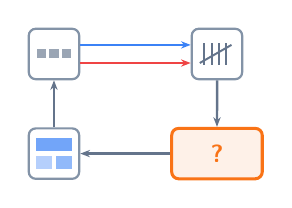
\begin{tikzpicture}[scale=1.15]
    \loopglyph{1}{3}
  \end{tikzpicture}}\\[12pt]
  {\normalsize\textcolor{grayout}{Jasper Gilley}}
\end{center}
\vfill
\end{frame}
}

% ══════════════════════════════════════════════════════════════════════════════
\section{The question}
% ══════════════════════════════════════════════════════════════════════════════

% ── Habit and value ───────────────────────────────────────────────────────────
\begin{frame}{Repetition builds habits whether or not they pay}
\begin{columns}[T]
\begin{column}{0.63\textwidth}
{\small A goal-directed learner repeats actions, and repetition turns them into \hltext{habits}.}

\smallskip
{\small Repetition does not check outcomes: a practised error becomes a habit as readily as a success.}

\smallskip
{\small Animals also have an \warmtext{evaluative system} that withholds reinforcement from repeated actions that do not pay.}

\smallskip
\begin{alertblock}{The question}
{\small In a learner that builds skills by repetition, when does a value gate in front of memory pay off, and can the learner grow it from its own practice? Here, memory is a \textbf{phrasebook} of reusable chunks.}
\end{alertblock}
\end{column}

\begin{column}{0.34\textwidth}
\centering
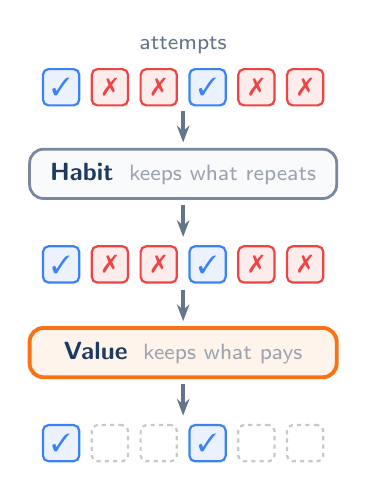
\begin{tikzpicture}[x=1cm,y=1cm]
  % attempts
  \foreach \i/\k in {0/P,1/F,2/F,3/P,4/F,5/F} {\csname Att\k\endcsname{\i*0.62}{3.55}}
  \node[note, anchor=south] at (1.55,3.85) {attempts};
  \draw[flow] (1.55,3.25) -- (1.55,2.85);
  % habit
  \node[organ, minimum width=3.9cm] (H) at (1.55,2.45)
      {\textbf{Habit} \;\dimtext{\footnotesize keeps what repeats}};
  \draw[flow] (1.55,2.05) -- (1.55,1.65);
  \foreach \i/\k in {0/P,1/F,2/F,3/P,4/F,5/F} {\csname Att\k\endcsname{\i*0.62}{1.3}}
  \draw[flow] (1.55,0.98) -- (1.55,0.58);
  % value
  \node[gateorgan, minimum width=3.9cm] (V) at (1.55,0.18)
      {\textbf{Value} \;\dimtext{\footnotesize keeps what pays}};
  \draw[flow] (1.55,-0.22) -- (1.55,-0.62);
  \foreach \i in {0,3} {\AttP{\i*0.62}{-0.97}}
  \foreach \i in {1,2,4,5} {\node[att, draw=grayout!60, dash pattern=on 1.5pt off 1.5pt] at (\i*0.62,-0.97) {};}
\end{tikzpicture}
\end{column}
\end{columns}
\end{frame}

% ══════════════════════════════════════════════════════════════════════════════
\section{A learner that practises}
% ══════════════════════════════════════════════════════════════════════════════

% ── The task ──────────────────────────────────────────────────────────────────
\begin{frame}{The task is to repair a damaged string so it derives its target again}
\begin{columns}[T]
\begin{column}{0.61\textwidth}
{\small A random \hltext{hierarchical grammar}: eight symbols per level, each with two rules that expand it into a pair one level down, six levels from root to 64 tokens. A level-$\ell$ node spans $2^\ell$ tokens.}

\smallskip
{\small A problem is a valid string for a \hltext{target} root with the span under one node \redtext{rewritten}, so it no longer derives the target. The learner edits it; a \hltext{grader} passes any valid derivation of the target.}

\smallskip
{\small A goal, attempts, and a graded outcome: goal-directed behaviour in miniature, with exact ground truth.}

\smallskip
\dimtext{\scriptsize Grammar: the Random Hierarchy Model (Cagnetta et al., 2024).}
\end{column}

\begin{column}{0.37\textwidth}
\centering
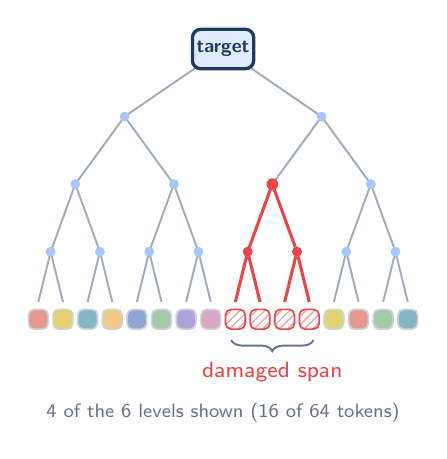
\begin{tikzpicture}[x=0.68cm,y=1.1cm]
  \def\dx{0.46}\def\dy{0.78}
  % edges
  \foreach \l in {1,2,3,4} {
    \pgfmathtruncatemacro{\n}{2^(4-\l)-1}
    \pgfmathtruncatemacro{\w}{2^\l}
    \pgfmathtruncatemacro{\wc}{2^(\l-1)}
    \foreach \j in {0,...,\n} {
      \pgfmathsetmacro{\xp}{(\j*\w + (\j+1)*\w - 1)/2*\dx}
      \pgfmathsetmacro{\xa}{((2*\j)*\wc + (2*\j+1)*\wc - 1)/2*\dx}
      \pgfmathsetmacro{\xb}{((2*\j+1)*\wc + (2*\j+2)*\wc - 1)/2*\dx}
      \pgfmathsetmacro{\yc}{\l==1 ? 0.2 : (\l-1)*\dy}
      \draw[streamgray!60, line width=0.7pt] (\xp,\l*\dy) -- (\xa,\yc);
      \draw[streamgray!60, line width=0.7pt] (\xp,\l*\dy) -- (\xb,\yc);
    }
  }
  % the damaged subtree (level-2 node over tokens 8–11)
  \draw[failc, line width=1.1pt] (4.37,1.56) -- (3.91,0.78) (4.37,1.56) -- (4.83,0.78);
  \draw[failc, line width=1.1pt] (3.91,0.78) -- (3.68,0.2) (3.91,0.78) -- (4.14,0.2);
  \draw[failc, line width=1.1pt] (4.83,0.78) -- (4.6,0.2) (4.83,0.78) -- (5.06,0.2);
  % internal nodes
  \foreach \l in {1,2,3} {
    \pgfmathtruncatemacro{\n}{2^(4-\l)-1}
    \pgfmathtruncatemacro{\w}{2^\l}
    \foreach \j in {0,...,\n} {
      \pgfmathsetmacro{\xp}{(\j*\w + (\j+1)*\w - 1)/2*\dx}
      \fill[mainblue!45] (\xp,\l*\dy) circle[radius=0.0625cm];
    }
  }
  \foreach \x in {3.91,4.83} {\fill[failc] (\x,0.78) circle[radius=0.0625cm];}
  \fill[failc] (4.37,1.56) circle[radius=0.074cm];
  \node[rootfeat, font=\sffamily\scriptsize\bfseries, minimum size=0.5cm] at (3.45,3.12) {target};
  % tokens
  \foreach \i/\c in {0/tokA,1/tokC,2/tokE,3/tokB,4/tokF,5/tokD,6/tokG,7/tokH,
                     12/tokC,13/tokA,14/tokD,15/tokE} {
    \node[tok, fill=\c, minimum size=0.25cm] at (\i*\dx,0) {};
  }
  \foreach \i in {8,9,10,11} {
    \node[tok, fill=failc!12, draw=failc, minimum size=0.25cm,
          pattern=north east lines, pattern color=failc!55] at (\i*\dx,0) {};
  }
  \draw[span] (3.6,-0.24) -- (5.14,-0.24);
  \node[note, text=failc, anchor=north] at (4.37,-0.38) {damaged span};
  \node[note, anchor=north, inner xsep=0pt] at (3.45,-0.85)
      {\scriptsize 4 of the 6 levels shown (16 of 64 tokens)};
\end{tikzpicture}
\end{column}
\end{columns}
\end{frame}

% ── The curriculum ────────────────────────────────────────────────────────────
\begin{frame}{The curriculum demands higher-level chunks}
\relax{\small The learner practises for \hltext{201 cycles} of 64 problems each. Stage $k$ damages a level-$k$ node, so the span to repair doubles: \textbf{2, 4, 8, 16, then 32 tokens}. Stage error is one minus that stage's held-out pass rate, averaged over its cycles.\par}

\smallskip
{\centering
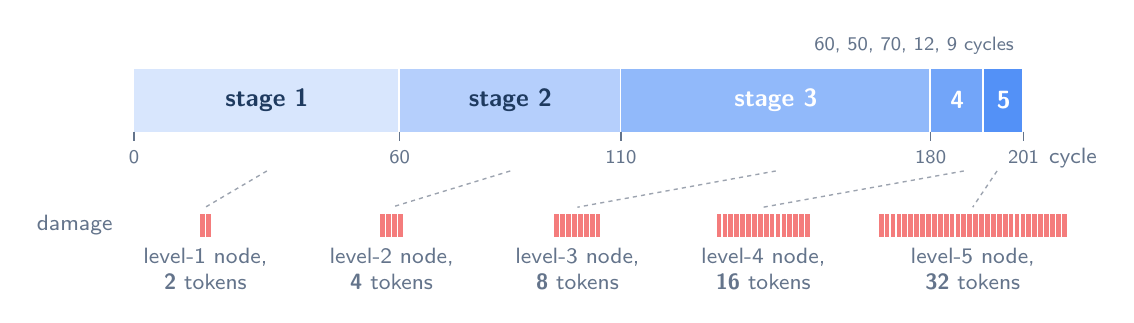
\begin{tikzpicture}[x=1cm,y=1cm]
  \def\cs{0.0562}  % cm per cycle: 201 cycles span 11.3cm
  \def\bh{0.8}     % band height
  % stage bands, each labelled inside its own band
  \foreach \a/\b/\c/\t/\l/\f in {0/60/lvlc0/maindark/stage 1/\small,
      60/110/lvlc1/maindark/stage 2/\small, 110/180/lvlc2/white/stage 3/\small,
      180/192/lvlc3/white/4/\small, 192/201/lvlc4/white/5/\small} {
    \fill[\c] (\a*\cs,0) rectangle (\b*\cs,\bh);
    \draw[white, line width=1pt] (\b*\cs,0) -- (\b*\cs,\bh);
    \node[font=\sffamily\f\bfseries, text=\t] at ({(\a+\b)/2*\cs},\bh/2) {\l};
  }
  % cycle axis
  \foreach \c in {0,60,110,180,201} {
    \draw[streamgray, line width=0.6pt] (\c*\cs,0) -- (\c*\cs,-0.12);
    \node[note, font=\sffamily\scriptsize, anchor=north] at (\c*\cs,-0.12) {\c};
  }
  \node[note, anchor=north west] at (201*\cs+0.2,-0.08) {cycle};
  % stage lengths, above the right end of the bar
  \node[note, anchor=south east, font=\sffamily\scriptsize] at (201*\cs,\bh+0.06)
      {60, 50, 70, 12, 9 cycles};
  % damaged span per stage
  \def\ty{-1.34}   % tile row bottom
  \foreach \k/\n/\cx in {1/2/0.905, 2/4/3.27, 3/8/5.63, 4/16/7.99, 5/32/10.65} {
    \pgfmathsetmacro{\w}{0.075}
    \pgfmathsetmacro{\xst}{\cx-\n*\w/2+\w*0.1}
    \foreach \t in {1,...,\n} {
      \fill[failc!70] ({\xst+(\t-1)*\w},\ty) rectangle ++(\w*0.8,0.3);
    }
    \node[note, anchor=north, align=center, inner sep=2pt] at (\cx,\ty-0.06)
      {level-\k{} node,\\\textbf{\n} tokens};
  }
  % leaders from bands to span rows (4 and 5 start off-centre in their bands, clear of the 180/201 labels)
  \foreach \mid/\cx in {30/0.905, 85/3.27, 145/5.63, 187.5/7.99, 195/10.65} {
    \draw[grayout, line width=0.5pt, dash pattern=on 1.5pt off 1.5pt]
      (\mid*\cs,-0.5) -- (\cx,\ty+0.38);
  }
  \node[note, anchor=east] at (-0.15,\ty+0.15) {damage};
\end{tikzpicture}\par}

\medskip
{\centering\footnotesize\dimtext{The last two stages give few cycles of evidence. Stage boundaries are the same at both seeds; when the learner may start using each level of chunks differs by seed.}\par}
\end{frame}

% ── The phrasebook ────────────────────────────────────────────────────────────
\begin{frame}{Chunks make large repairs possible; a missing half blocks the levels above}
\begin{columns}[T]
\begin{column}{0.45\textwidth}
Repairing 32 tokens one token at a time exceeds the search planner's budget. \hltext{Chunks} let it compose large repairs from a few reusable pieces.

\medskip
{\small The \hltext{phrasebook} is organised by level. The level-1 chunks, the eight bottom symbols, are given; each spans 2 tokens. Above that, every level-$\ell$ chunk is a pair of level-$(\ell{-}1)$ chunks and must be \textbf{earned}.}

\end{column}

\begin{column}{0.53\textwidth}
\centering
\resizebox{\linewidth}{!}{%
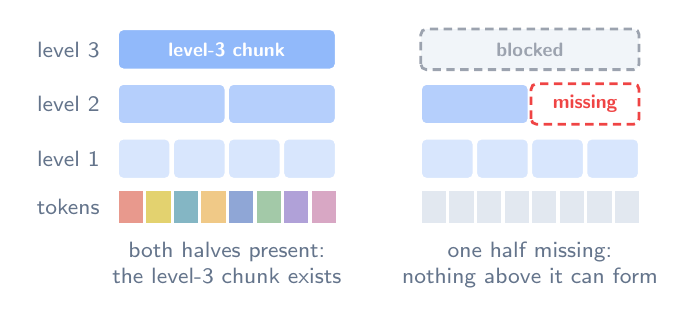
\begin{tikzpicture}[x=0.7cm,y=1.12cm]
  \def\bh{0.46}
  % level labels
  \foreach \l/\y in {1/0, 2/0.62, 3/1.24} {
    \node[note, anchor=east] at (-0.15,\y+\bh/2) {level \l};
  }
  % tokens
  \foreach \i/\c in {0/tokA,1/tokC,2/tokE,3/tokB,4/tokF,5/tokD,6/tokG,7/tokH} {
    \fill[\c] (\i*0.5+0.02,-0.5) rectangle ++(0.44,0.36);
  }
  \node[note, anchor=east] at (-0.15,-0.32) {tokens};
  % complete stack
  \foreach \x in {0,1,2,3} {\fill[lvlc0, chunk] (\x,0) rectangle ++(0.96,\bh);}
  \foreach \x in {0,2} {\fill[lvlc1, chunk] (\x,0.62) rectangle ++(1.96,\bh);}
  \fill[lvlc2, chunk] (0,1.24) rectangle ++(3.96,\bh);
  \node[font=\sffamily\scriptsize\bfseries, text=white] at (1.98,1.24+\bh/2) {level-3 chunk};
  \node[note, anchor=north, align=center] at (1.98,-0.6) {both halves present:\\ the level-3 chunk exists};
  % blocked stack
  \begin{scope}[shift={(5.5,0)}]
    \foreach \t in {0,...,7} {\fill[slate200] (\t*0.5+0.02,-0.5) rectangle ++(0.44,0.36);}
    \foreach \x in {0,1,2,3} {\fill[lvlc0, chunk] (\x,0) rectangle ++(0.96,\bh);}
    \fill[lvlc1, chunk] (0,0.62) rectangle ++(1.96,\bh);
    \draw[warmred, line width=1pt, dash pattern=on 3pt off 2pt, rounded corners=2pt]
        (2,0.62) rectangle ++(1.96,\bh);
    \node[font=\sffamily\scriptsize\bfseries, text=warmred] at (2.98,0.62+\bh/2) {missing};
    \draw[grayout, line width=1pt, dash pattern=on 3pt off 2pt, rounded corners=2pt, fill=slate100]
        (0,1.24) rectangle ++(3.96,\bh);
    \node[font=\sffamily\scriptsize\bfseries, text=grayout] at (1.98,1.24+\bh/2) {blocked};
    \node[note, anchor=north, align=center] at (1.98,-0.6) {one half missing:\\ nothing above it can form};
  \end{scope}
\end{tikzpicture}}

\medskip
\begin{block}{Nesting cuts both ways}
{\small A level-3 chunk requires both level-2 halves. A missing half \textbf{blocks} everything that would be built on it.}
\end{block}
\end{column}
\end{columns}
\end{frame}

% ── The habit counter ─────────────────────────────────────────────────────────
\begin{frame}{The habit counter grows the phrasebook by repetition}
\begin{columns}[T]
\begin{column}{0.45\textwidth}
{\small After each cycle the counter tallies pairings around each repair: the repaired level-$k$ span and its neighbour form a candidate level-$(k{+}1)$ chunk. It works \hltext{one level ahead}.\par}

\smallskip
{\small A pairing seen \textbf{three times} is offered to the phrasebook, even before its level is usable: level-2 chunks enter in stage 1 and are first written at cycle 48 / 59.\par}

\smallskip
\begin{block}{By default}
{\small Only \textbf{successful} repairs count. Unlike habit, this counter checks outcomes.\par}
\end{block}
\end{column}

\begin{column}{0.52\textwidth}
\centering
\resizebox{\linewidth}{!}{%
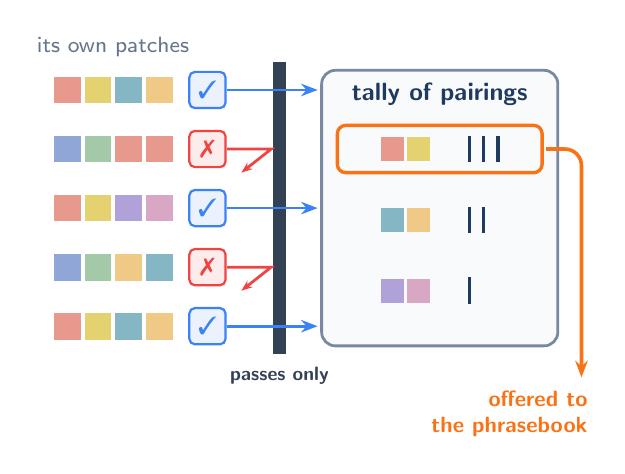
\begin{tikzpicture}[x=1cm,y=1cm]
  % patches
  \node[note, anchor=south] at (0.75,3.3) {its own patches};
  \foreach \y/\k/\ca/\cb/\cc/\cd in {3.0/P/tokA/tokC/tokE/tokB, 2.25/F/tokF/tokD/tokA/tokA,
      1.5/P/tokA/tokC/tokG/tokH, 0.75/F/tokF/tokD/tokB/tokE, 0.0/P/tokA/tokC/tokE/tokB} {
    \foreach \c [count=\t] in {\ca,\cb,\cc,\cd} {\fill[\c] ({(\t-1)*0.39},\y-0.17) rectangle ++(0.34,0.34);}
    \csname Att\k\endcsname{1.95}{\y}
  }
  % filter
  \fill[slate700] (2.78,-0.35) rectangle (2.95,3.35);
  \node[note, anchor=north, text=slate700, font=\sffamily\scriptsize\bfseries]
      at (2.865,-0.4) {passes only};
  \foreach \y in {3.0,1.5,0.0} {\draw[flow, color=passc, line width=1pt] (2.2,\y) -- (3.35,\y);}
  \foreach \y in {2.25,0.75} {
    \draw[failc, line width=1pt, -{Stealth[length=4pt]}] (2.2,\y) -- (2.76,\y) -- (2.38,\y-0.3);
  }
  % tally board
  \node[organ, minimum width=3.0cm, minimum height=3.5cm] (T) at (4.9,1.5) {};
  \node[caphead, font=\sffamily\small\bfseries] at (4.9,2.95) {tally of pairings};
  \foreach \y/\ca/\cb/\n in {2.25/tokA/tokC/3, 1.35/tokE/tokB/2, 0.45/tokG/tokH/1} {
    \fill[\ca] (4.15,\y-0.15) rectangle ++(0.3,0.3);
    \fill[\cb] (4.48,\y-0.15) rectangle ++(0.3,0.3);
    \foreach \t in {1,...,\n} {\draw[maindark, line width=1.1pt] ({5.1+\t*0.18},\y-0.17) -- ++(0,0.34);}
  }
  \draw[gateorange, line width=1.2pt, rounded corners=3pt] (3.6,1.95) rectangle (6.2,2.55);
  \draw[flow, color=gateorange, rounded corners=6pt] (6.25,2.25) -- (6.7,2.25) -- (6.7,-0.65);
  \node[emph, anchor=north east, align=right] at (6.9,-0.7) {offered to\\the phrasebook};
\end{tikzpicture}}
\end{column}
\end{columns}
\end{frame}

% ── The value gate ────────────────────────────────────────────────────────────
\begin{frame}{The value gate admits chunks first, then tests what can be built on them}
\begin{columns}[T]
\begin{column}{0.38\textwidth}
{\small A chunk's worth must be tested, so every offered chunk enters \warmtext{provisionally}. Its job is to be built on, so it is judged through its \hltext{consumers}: pairings one level up that contain it.}

\medskip
{\small Each consumer is \hltext{tried alone} on 192 fresh problems damaged at its level, using only that chunk. Unrepaired, they pass at 0, so its gain is its pass rate.}
\end{column}

\begin{column}{0.60\textwidth}
\centering
\resizebox{\linewidth}{!}{%
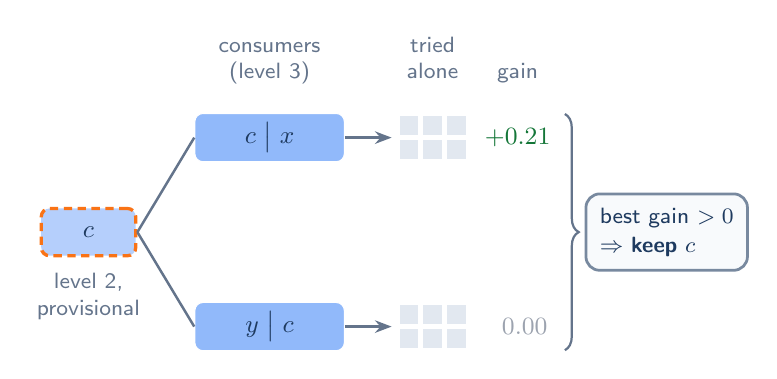
\begin{tikzpicture}[x=1cm,y=1cm]
  % the provisional chunk
  \node[draw=gateorange, dash pattern=on 3pt off 2pt, line width=1.2pt, fill=lvlc1,
        rounded corners=3pt, minimum width=1.2cm, minimum height=0.6cm,
        font=\sffamily\small\bfseries, text=maindark] (c) at (0,0) {$c$};
  \node[note, anchor=north, align=center] at (0,-0.4) {level 2,\\ provisional};
  % consumers
  \foreach \y/\l/\r/\n in {1.2/$c$/$x$/1, -1.2/$y$/$c$/2} {
    \node[draw=white, fill=lvlc2, rounded corners=3pt, minimum width=1.9cm,
          minimum height=0.6cm, font=\sffamily\small\bfseries, text=maindark] (k\n) at (2.3,\y) {\l\;\big|\;\r};
    \draw[streamgray, line width=0.9pt] (c.east) -- (k\n.west);
  }
  % tried alone on fresh problems
  \foreach \n/\y in {1/1.2, 2/-1.2} {
    \draw[flow, line width=1pt] (k\n.east) -- (3.85,\y);
    \foreach \a in {0,1,2} {\foreach \b in {0,1} {
      \fill[slate200] ({3.95+\a*0.3},{\y-0.27+\b*0.3}) rectangle ++(0.24,0.24);}}
  }
  \node[font=\sffamily\small\bfseries, text=armoracle] at (5.45,1.2) {$+0.21$};
  \node[font=\sffamily\small\bfseries, text=grayout] at (5.45,-1.2) {$\;\;0.00$};
  % column headers, one shared baseline
  \foreach \x/\t in {2.3/{consumers\\(level 3)}, 4.37/{tried\\alone}, 5.45/{gain}}
    \node[note, anchor=base, align=center] at (\x,1.95) {\t};
  % decision
  \draw[decorate, decoration={brace, amplitude=5pt}, line width=0.8pt, streamgray] (6.05,1.5) -- (6.05,-1.5);
  \node[organ, anchor=west, align=left, font=\sffamily\footnotesize] at (6.3,0)
      {best gain $>0$\\[1pt] $\Rightarrow$ \textbf{keep} $c$};
\end{tikzpicture}}

\medskip
{\footnotesize
\setlength{\leftmargini}{1.05em}\begin{itemize}\itemsep1pt
  \item No consumer with positive gain: \textbf{remove}.
  \item No consumer within a timer: \textbf{remove} \dimtext{(a known flaw, kept)}.
  \item A new consumer enters the tally later: \textbf{offer again}.
\end{itemize}}
\end{column}
\end{columns}
\end{frame}

% ── Two graders ───────────────────────────────────────────────────────────────
\begin{frame}{Either the oracle or the learner's own read can judge chunks}
\begin{center}
\resizebox{0.96\linewidth}{!}{%
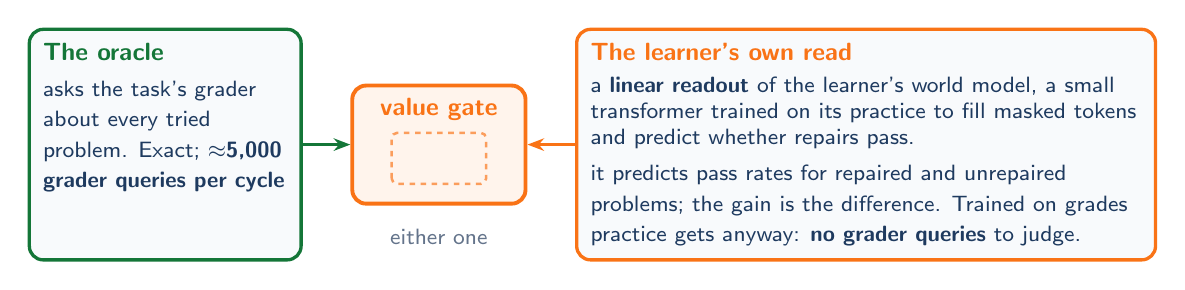
\begin{tikzpicture}[x=1cm,y=1cm]
  % the gate slot
  \node[gateorgan, minimum width=2.2cm, minimum height=1.5cm] (G) at (0,0) {};
  \node[font=\sffamily\small\bfseries, text=gateorange] at (0,0.45) {value gate};
  \draw[gateorange!70, dash pattern=on 2pt off 2pt, line width=0.9pt, rounded corners=2pt]
      (-0.6,-0.5) rectangle (0.6,0.15);
  % own read
  \node[organ, draw=armread, line width=1.2pt, text width=7.0cm, align=flush left, anchor=west, outer sep=0pt] (R) at (1.75,0)
    {\textcolor{armread}{\textbf{The learner's own read}}\\[2pt]
     \footnotesize a \textbf{linear readout} of the learner's world model, a small transformer trained on its practice to fill masked tokens and predict whether repairs pass.\\[2pt]
     \footnotesize it predicts pass rates for repaired and unrepaired problems; the gain is the difference. Trained on grades practice gets anyway: \textbf{no grader queries} to judge.};
  % oracle: same height as the read card, heading aligned with it
  \node[organ, draw=none, fill=none, text width=3.1cm, align=flush left, anchor=north east, outer sep=0pt] (Ot) at (-1.75,0 |- R.north)
    {\textcolor{armoracle}{\textbf{The oracle}}\\[2pt]
     \footnotesize asks the task's grader about every tried problem. Exact; \textbf{$\approx$5{,}000 grader queries per cycle}};
  \begin{scope}[on background layer]
    \node[organ, draw=armoracle, line width=1.2pt, inner sep=0pt, outer sep=0pt, fit=(Ot.north west) (Ot.east |- R.south)] (O) {};
  \end{scope}
  \draw[flow, color=armoracle] (O.east) -- (G.west);
  \draw[flow, color=armread] (R.west) -- (G.east);
  \node[note, anchor=north] at (0,-0.95) {either one};
\end{tikzpicture}}
\end{center}

\medskip
\begin{center}
{\small The read waits for \warmtext{512 of its own graded writes} at the consumers' level before judging.}
\end{center}
\end{frame}

% ══════════════════════════════════════════════════════════════════════════════
\section{Two ways of counting}
% ══════════════════════════════════════════════════════════════════════════════

% ── Successes only ────────────────────────────────────────────────────────────
\begin{frame}{When only successes count, a value gate has nothing to add}
\begin{columns}[T]
\begin{column}{0.55\textwidth}
{\small With successes-only counting, even the \oracletext{oracle} gate does no better than no gate, at either seed.}

\smallskip
{\small What recurs in successes is mostly worth keeping: frequency is a close stand-in for value. The limit is how fast true chunks \emph{arrive}, not the quality of what gets in.}

\smallskip
\begin{alertblock}{Takeaway}
{\small The success filter already does a value system's job. Real habit doesn't check outcomes, so no real learner has this filter built in.}
\end{alertblock}
\end{column}

\begin{column}{0.43\textwidth}
\centering
\resizebox{\linewidth}{!}{%
\begin{tikzpicture}[x=1cm,y=1cm]
  \def\ys{11.5}
  % local copy of \dpanel: the two bars of a stage 0.1 apart (not 0.02) and the
  % seed-2 value labels nudged right (seed-0 left), so they clear the neighbouring bar
  \renewcommand{\dpanel}[6]{%
    \begin{scope}[shift={(####1,0)}]
      \draw[streamgray, line width=0.7pt] (0,0) -- (4.6,0);
      \foreach \v [count=\i] in {####3} {
        \pgfmathsetmacro{\xx}{(\i-1)*1.1+0.24}
        \fill[####5] (\xx,0) rectangle ++(0.36,{\v*\ys});
        \pgfmathsetmacro{\yl}{\v>=0 ? \v*\ys+0.14 : \v*\ys-0.14}
        \node[valnum] at (\xx+0.10,\yl) {\sgnum{\v}};
      }
      \foreach \v [count=\i] in {####4} {
        \pgfmathsetmacro{\xx}{(\i-1)*1.1+0.70}
        \fill[####6] (\xx,0) rectangle ++(0.36,{\v*\ys});
        \pgfmathsetmacro{\yl}{\v>=0 ? \v*\ys+0.14 : \v*\ys-0.14}
        \node[valnum] at (\xx+0.25,\yl) {\sgnum{\v}};
      }
    \end{scope}}
  % y grid
  \foreach \t in {-0.1,0.1,0.2} {
    \draw[slate200, line width=0.5pt] (-0.1,\t*\ys) -- (4.6,\t*\ys);
    \node[note, font=\sffamily\scriptsize, anchor=east] at (-0.1,\t*\ys)
        {\pgfmathprintnumber[fixed,precision=1,showpos]{\t}};
  }
  \node[note, font=\sffamily\scriptsize, anchor=east] at (-0.1,0) {0};
  \node[note, rotate=90, anchor=south, align=center] at (-0.82,{0.05*\ys})
      {error, oracle gate $-$ no gate};
  \dpanel{0}{}{-0.002,0.035,0.176,0.053}{-0.033,-0.002,0.016,0.008}{armoracle}{armoracle!40}
  \dstages{0}{-0.1}
  \node[note, font=\sffamily\scriptsize, align=center] (neg) at (2.3,{-0.1*\ys-1.05}) {negative: the gate helps};
  \node[note, font=\sffamily\tiny, align=center, text=grayout, text width=4.7cm, anchor=north, inner sep=1pt] at ([yshift=-1pt]neg.south) {stage 1 omitted: earned chunks are unusable for most of it, and all conditions agree within 0.005};
  \node[note, font={\sffamily\scriptsize\baselineskip=9pt}, anchor=north east, text=grayout, align=right, inner sep=1pt, fill=white] at (2.37,{0.176*\ys})
      {the timer: removed\\a level-3 chunk\\that five level-4\\chunks needed};
  % legend
  \fill[armoracle] (0.1,{0.2*\ys+0.51}) rectangle ++(0.22,0.18);
  \node[note, anchor=west, font=\sffamily\scriptsize] at (0.35,{0.2*\ys+0.6}) {seed 0};
  \fill[armoracle!40] (1.55,{0.2*\ys+0.51}) rectangle ++(0.22,0.18);
  \node[note, anchor=west, font=\sffamily\scriptsize] at (1.8,{0.2*\ys+0.6}) {seed 2};
  % glyph badge
  \begin{scope}[shift={(3.33,{0.2*\ys+0.3})}, x=1cm, scale=0.55, transform shape, name prefix=b-]
    \loopglyph{0}{1}
  \end{scope}
\end{tikzpicture}}
\end{column}
\end{columns}
\end{frame}

% ── The one change ────────────────────────────────────────────────────────────
\begin{frame}{One change blinds the counter to outcome: count the failures too}
\relax{\small The counter still samples successful repairs exactly as before. It now also counts \redtext{failed repairs}, in the batch's own ratio: about \textbf{three failures for every success}.\par}

\smallskip
{\centering
\resizebox{0.9\linewidth}{!}{%
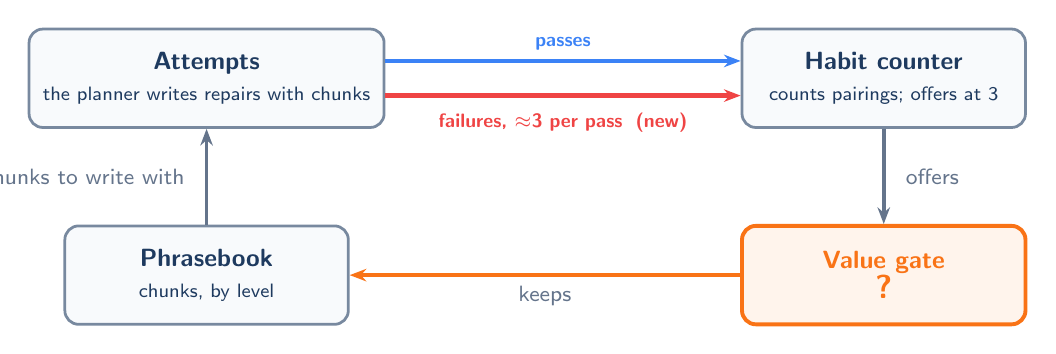
\begin{tikzpicture}[x=1cm,y=1cm]
  \node[organ, minimum width=3.6cm, minimum height=1.25cm] (A) at (0,2.5)
      {\textbf{Attempts}\\ \scriptsize the planner writes repairs with chunks};
  \node[organ, minimum width=3.6cm, minimum height=1.25cm] (C) at (8.6,2.5)
      {\textbf{Habit counter}\\ \scriptsize counts pairings; offers at 3};
  \node[gateorgan, minimum width=3.6cm, minimum height=1.25cm] (G) at (8.6,0)
      {\textbf{\textcolor{gateorange}{Value gate}}\\ \large\textbf{\textcolor{gateorange}{?}}};
  \node[organ, minimum width=3.6cm, minimum height=1.25cm] (P) at (0,0)
      {\textbf{Phrasebook}\\ \scriptsize chunks, by level};
  \draw[flow, color=passc] ($(A.east)+(0,0.22)$) -- node[above, font=\sffamily\scriptsize\bfseries, text=passc] {passes} ($(C.west)+(0,0.22)$);
  \draw[flow, color=failc, line width=1.7pt] ($(A.east)+(0,-0.22)$) -- node[below=2pt, font=\sffamily\scriptsize\bfseries, text=failc] {failures, $\approx$3 per pass \;(new)} ($(C.west)+(0,-0.22)$);
  \draw[flow] (C) -- node[right=4pt, note] {offers} (G);
  \draw[flow, color=gateorange] (G) -- node[below, note] {keeps} (P);
  \draw[flow] (P) -- node[left=4pt, note, overlay] {chunks to write with} (A);
\end{tikzpicture}}\par}

\smallskip
{\centering\footnotesize
\dimtext{Everything else is the same: grammar, planner, world model, and each seed's schedule of when chunk levels become usable. Gated runs branch from the ungated run at cycle 10 / 5, before any chunk is judged.}\par}
\end{frame}

% ── The junk ──────────────────────────────────────────────────────────────────
\begin{frame}{The junk is the learner's own recurring mistakes}
\begin{columns}[T]
\begin{column}{0.43\textwidth}
{\footnotesize The counter sees only the region around a repair, so a failure contributes \redtext{exactly its wrong patch}; at three failures per success, the most-repeated patches are errors.\par}

\smallskip
{\footnotesize By cycle 40 the level-2 counter holds 47 and 48 chunks (seeds 0 and 2), against 13 counting successes alone. Of the newcomers, 29 and 30 are not in the grammar; tried alone, \textbf{28 of 29} and \textbf{30 of 30} repair nothing. Added to the phrasebook so far, a quarter to a third make it worse.\par}

\smallskip
{\footnotesize True chunks are not delayed: all 14 the run finds arrive by cycle 50 / 25.\par}
\end{column}

\begin{column}{0.55\textwidth}
\centering
\resizebox{\linewidth}{!}{%
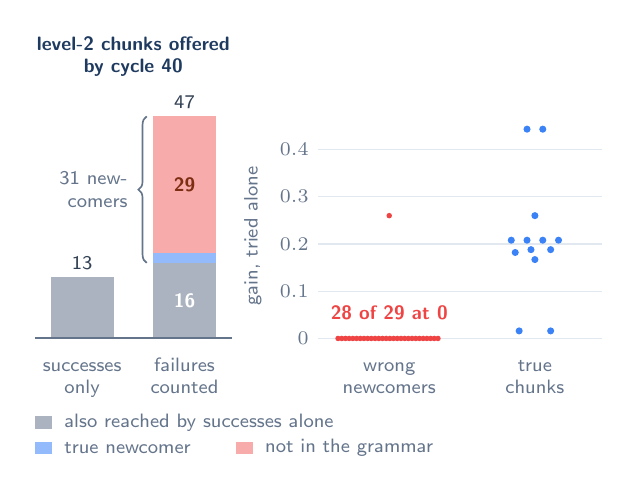
\begin{tikzpicture}[x=1cm,y=1cm]
  % left: chunks offered by cycle 40 (seed 0)
  \def\cy{0.06}
  \fill[armref!55] (0.2,0) rectangle ++(0.8,13*\cy);
  \node[valnum, font=\sffamily\scriptsize] at (0.6,13*\cy+0.18) {13};
  \fill[armref!55] (1.5,0) rectangle ++(0.8,16*\cy);
  \fill[truec] (1.5,16*\cy) rectangle ++(0.8,2*\cy);
  \fill[falsec] (1.5,18*\cy) rectangle ++(0.8,29*\cy);
  \node[font=\sffamily\scriptsize\bfseries, text=white] at (1.9,8*\cy) {16};
  \node[font=\sffamily\scriptsize\bfseries, text=gatedark] at (1.9,32.5*\cy) {29};
  \node[valnum, font=\sffamily\scriptsize] at (1.9,47*\cy+0.18) {47};
  \draw[decorate, decoration={brace, amplitude=3pt}, line width=0.6pt, streamgray]
      (1.42,16*\cy) -- (1.42,47*\cy);
  \node[note, font=\sffamily\scriptsize, anchor=east, align=right] at (1.3,31.5*\cy) {31 new-\\comers};
  \draw[streamgray, line width=0.7pt] (0,0) -- (2.5,0);
  \node[note, anchor=base, align=center, font=\sffamily\scriptsize] at (0.6,-0.70) {successes\\only};
  \node[note, anchor=base, align=center, font=\sffamily\scriptsize] at (1.9,-0.70) {failures\\counted};
  \node[caphead, font=\sffamily\scriptsize\bfseries, align=center] at (1.25,3.58) {level-2 chunks offered\\by cycle 40};
  % legend
  \fill[armref!55] (0.0,-1.15) rectangle ++(0.22,0.16); \node[note, anchor=west, font=\sffamily\scriptsize] at (0.25,-1.07) {also reached by successes alone};
  \fill[truec] (0.0,-1.47) rectangle ++(0.22,0.16); \node[note, anchor=west, font=\sffamily\scriptsize] at (0.25,-1.39) {true newcomer};
  \fill[falsec] (2.55,-1.47) rectangle ++(0.22,0.16); \node[note, anchor=west, font=\sffamily\scriptsize] at (2.8,-1.39) {not in the grammar};
  % right: tried-alone gains
  \begin{scope}[shift={(3.6,0)}]
    \def\gy{6}
    \foreach \t in {0,0.1,0.2,0.3,0.4} {
      \draw[slate200, line width=0.5pt] (0,\t*\gy) -- (3.6,\t*\gy);
      \node[note, font=\sffamily\scriptsize, anchor=east] at (0,\t*\gy) {\pgfmathprintnumber[fixed,precision=1]{\t}};
    }
    \node[note, rotate=90, anchor=south, font=\sffamily\scriptsize] at (-0.6,1.3) {gain, tried alone};
    % wrong newcomers: 28 at 0, one at 0.26
    \foreach \k in {0,...,27} {\fill[failc] ({0.25+\k*0.047},0) circle (0.035);}
    \fill[failc] (0.9,0.26*\gy) circle (0.035);
    % true chunks
    \foreach \g/\dxx in {0.016/-0.2, 0.016/0.2, 0.167/0, 0.182/-0.25, 0.188/0.2, 0.188/-0.05,
        0.208/-0.3, 0.208/-0.1, 0.208/0.1, 0.208/0.3, 0.26/0, 0.443/-0.1, 0.443/0.1} {
      \fill[passc] ({2.75+\dxx},\g*\gy) circle (0.045);
    }
    \node[note, anchor=base, align=center, font=\sffamily\scriptsize] at (0.9,-0.70) {wrong\\newcomers};
    \node[note, anchor=base, align=center, font=\sffamily\scriptsize] at (2.75,-0.70) {true\\chunks};
    \node[note, text=failc, font=\sffamily\scriptsize\bfseries, anchor=south] at (0.9,0.12) {28 of 29 at 0};
  \end{scope}
\end{tikzpicture}}

{\tiny\dimtext{seed 0, cycle 40. Labels compare spellings with the grammar's rules; a few legal chunks spell like illegal ones (one labelled false repairs 26\%).}\par}
\end{column}
\end{columns}
\end{frame}

% ── Ungated ───────────────────────────────────────────────────────────────────
\begin{frame}{Without a gate, the learner memorises its mistakes and loses depth}
\relax{\small The ungated phrasebook ends several times larger than the successes-only one, at about a third of its precision (the share labelled true): at level 2, \textbf{61 chunks at 0.23} against \textbf{17 at 0.65} (seed 0). As damage spans grow, error rises stage by stage above the successes-only learner.}

\medskip
\begin{center}
\resizebox{0.95\linewidth}{!}{%
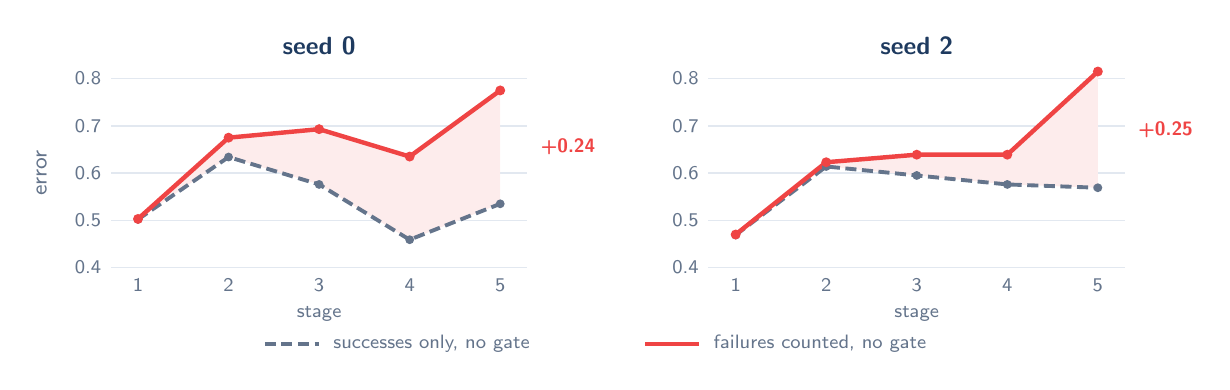
\begin{tikzpicture}[x=1.15cm,y=6cm]
  \foreach \px/\seed/\ra/\rb/\rc/\rd/\re/\fa/\fb/\fc/\fd/\fe/\gap in {
      0/seed 0/.502/.634/.576/.459/.535/.503/.675/.693/.635/.775/+0.24,
      6.6/seed 2/.469/.614/.595/.576/.569/.470/.623/.639/.639/.815/+0.25} {
    \begin{scope}[shift={(\px,-0.4)}]
      \foreach \t in {0.4,0.5,0.6,0.7,0.8} {
        \draw[slate200, line width=0.5pt] (0.7,\t) -- (5.3,\t);
        \node[note, font=\sffamily\scriptsize, anchor=east] at (0.7,\t) {\t};
      }
      \fill[failc!10] (1,\ra) -- (2,\rb) -- (3,\rc) -- (4,\rd) -- (5,\re) --
                      (5,\fe) -- (4,\fd) -- (3,\fc) -- (2,\fb) -- (1,\fa) -- cycle;
      \draw[armref, line width=1.4pt, dash pattern=on 4pt off 2pt]
          (1,\ra) -- (2,\rb) -- (3,\rc) -- (4,\rd) -- (5,\re);
      \draw[armfloor, line width=1.6pt] (1,\fa) -- (2,\fb) -- (3,\fc) -- (4,\fd) -- (5,\fe);
      \foreach \x/\y in {1/\ra,2/\rb,3/\rc,4/\rd,5/\re} {\fill[armref] (\x,\y) circle (1.6pt);}
      \foreach \x/\y in {1/\fa,2/\fb,3/\fc,4/\fd,5/\fe} {\fill[armfloor] (\x,\y) circle (1.8pt);}
      \foreach \s in {1,...,5} {\node[note, font=\sffamily\scriptsize] at (\s,0.362) {\s};}
      \node[note, font=\sffamily\scriptsize] at (3,0.302) {stage};
      \node[caphead, font=\sffamily\small\bfseries] at (3,0.87) {\seed};
      \node[font=\sffamily\scriptsize\bfseries, text=armfloor, anchor=west] at (5.34,{(\re+\fe)/2}) {\gap};
    \end{scope}
  }
  \node[note, rotate=90, anchor=south] at (0.1,0.2) {error};
  % legend
  \draw[armref, line width=1.4pt, dash pattern=on 4pt off 2pt] (2.4,-0.162) -- ++(0.6,0);
  \node[note, anchor=west, font=\sffamily\scriptsize] at (3.05,-0.162) {successes only, no gate};
  \draw[armfloor, line width=1.6pt] (6.6,-0.162) -- ++(0.6,0);
  \node[note, anchor=west, font=\sffamily\scriptsize] at (7.25,-0.162) {failures counted, no gate};
\end{tikzpicture}}
\end{center}
\end{frame}

% ══════════════════════════════════════════════════════════════════════════════
\section{The value gate at work}
% ══════════════════════════════════════════════════════════════════════════════

% ── The oracle rebuilds the vocabulary ────────────────────────────────────────
\begin{frame}{The oracle gate rebuilds the phrasebook from the polluted stream}
\begin{columns}[T]
\begin{column}{0.36\textwidth}
{\small The \oracletext{oracle} gate cuts the level-2 phrasebook to 17 chunks by cycle 40, the successes-only learner's final size. It ends with \textbf{14 true} and \textbf{5 false}, against 14 and 47 ungated (seed 0).\par}

\smallskip
{\small None of its \textbf{542 removals} (both seeds, by timer or by value) is of a chunk labelled true.\par}

\smallskip
{\small It beats the ungated run in 3 of 4 stages at seed 0 and 4 of 4 at seed 2, at $\approx$5{,}000 grader queries per cycle.\par}
\end{column}

\begin{column}{0.62\textwidth}
\centering
\resizebox{\linewidth}{!}{%
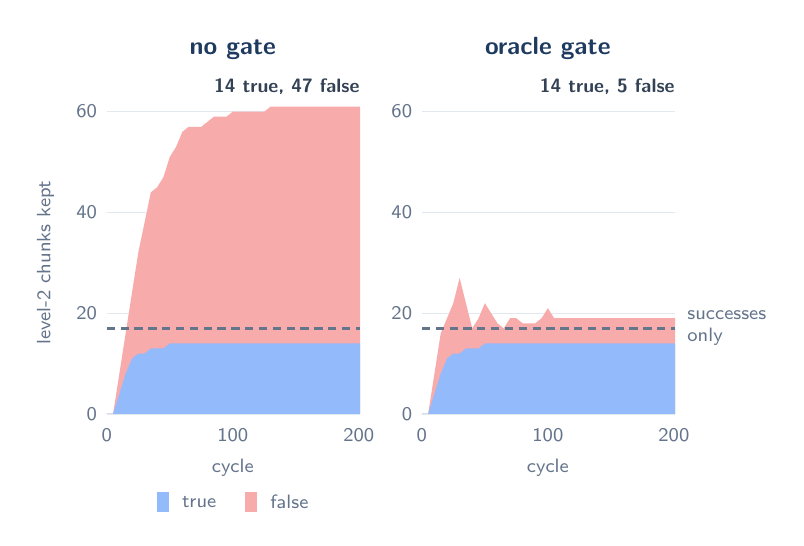
\begin{tikzpicture}[x=0.016cm,y=0.064cm]
  \foreach \px/\ttl/\tot/\tru/\lab in {0/no gate/\serAfloortot/\serAfloortru/{14 true, 47 false},
                                    250/oracle gate/\serAoracletot/\serAoracletru/{14 true, 5 false}} {
    \begin{scope}[shift={(\px,0)}]
      \foreach \t in {0,20,40,60} {
        \draw[slate200, line width=0.5pt] (0,\t) -- (201,\t);
        \node[note, font=\sffamily\scriptsize, anchor=east] at (0,\t) {\t};
      }
      \fill[falsec] \tot -- (201,0) -- cycle;
      \fill[truec] \tru -- (201,0) -- cycle;
      \draw[armref, line width=1pt, dash pattern=on 3pt off 2pt] (0,17) -- (201,17);
      \foreach \c in {0,100,200} {\node[note, font=\sffamily\scriptsize, anchor=north] at (\c,-1) {\c};}
      \node[note, font=\sffamily\scriptsize, anchor=north] at (100,-7) {cycle};
      \node[caphead, font=\sffamily\small\bfseries, anchor=south] at (100,68.5) {\ttl};
      \node[note, font=\sffamily\scriptsize\bfseries, text=slate700, anchor=south east, inner xsep=0pt] at (201,61.5) {\lab};
    \end{scope}
  }
  \node[note, font=\sffamily\scriptsize, anchor=west, align=left, text=armref] at (453,17) {successes\\only};
  \node[note, rotate=90, anchor=south, font=\sffamily\scriptsize] at (-34,30) {level-2 chunks kept};
  % legend
  \fill[truec] (40,-19.5) rectangle ++(9,4); \node[note, anchor=west, font=\sffamily\scriptsize] at (52,-17.5) {true};
  \fill[falsec] (110,-19.5) rectangle ++(9,4); \node[note, anchor=west, font=\sffamily\scriptsize] at (122,-17.5) {false};
\end{tikzpicture}}

\dimtext{\scriptsize seed 0}
\end{column}
\end{columns}
\end{frame}

% ── The same grader, two ways of counting ─────────────────────────────────────
\begin{frame}{A value gate's payoff depends on what the counter filters out upstream}
\relax{\small The oracle grades every trial exactly, so it shows whether the gate can help at all. Counting only successes, it adds nothing. When failures count, it closes the gap to the successes-only learner at stages 2--3 on both seeds and stage 4 at seed 2, but not at the last stage.}

\smallskip
{\centering
\resizebox{0.86\linewidth}{!}{%
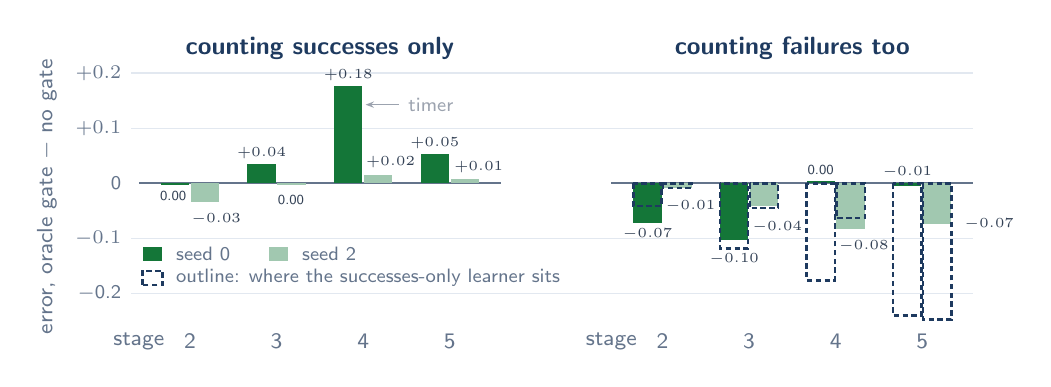
\begin{tikzpicture}[x=1cm,y=1cm]
  % Panels drawn locally (same geometry and styles as \dpanel/\dstages) so each
  % value label can sit clear of the bars and of the dashed outline bars.
  \def\ys{7}
  \foreach \t in {-0.1,0.1,0.2} {
    \draw[slate200, line width=0.5pt] (-0.1,\t*\ys) -- (10.6,\t*\ys);
    \node[note, font=\sffamily\scriptsize, anchor=east] at (-0.1,\t*\ys)
        {\pgfmathprintnumber[fixed,precision=1,showpos]{\t}};
  }
  \node[note, font=\sffamily\scriptsize, anchor=east] at (-0.1,0) {0};
  \node[note, rotate=90, anchor=south, align=center] at (-0.92,-0.17) {error, oracle gate $-$ no gate};
  \draw[slate200, line width=0.5pt] (-0.1,-0.2*\ys) -- (10.6,-0.2*\ys);
  \node[note, font=\sffamily\scriptsize, anchor=east] at (-0.1,-0.2*\ys) {$-$0.2};
  % bars (seed 0 at +0.28, seed 2 at +0.66 in each 1.1-wide stage slot)
  \foreach \px/\A/\B in {0/{-0.002,0.035,0.176,0.053}/{-0.033,-0.002,0.016,0.008},
                         6/{-0.071,-0.103,0.004,-0.005}/{-0.008,-0.041,-0.083,-0.074}} {
    \begin{scope}[shift={(\px,0)}]
      \draw[streamgray, line width=0.7pt] (0,0) -- (4.6,0);
      \foreach \v [count=\i] in \A {\fill[armoracle] ({(\i-1)*1.1+0.28},0) rectangle ++(0.36,{\v*\ys});}
      \foreach \v [count=\i] in \B {\fill[armoracle!40] ({(\i-1)*1.1+0.66},0) rectangle ++(0.36,{\v*\ys});}
    \end{scope}}
  \node[caphead, font=\sffamily\small\bfseries] at (2.3,1.72) {counting successes only};
  \node[caphead, font=\sffamily\small\bfseries] at (8.3,1.72) {counting failures too};
  % where the successes-only learner sits, relative to no gate (failures counted)
  \begin{scope}[shift={(6,0)}]
    \foreach \v [count=\i] in {-0.041,-0.118,-0.176,-0.240} {
      \draw[maindark, line width=0.9pt, dash pattern=on 2pt off 1.2pt] ({(\i-1)*1.1+0.28},0) rectangle ++(0.36,{\v*\ys});}
    \foreach \v [count=\i] in {-0.008,-0.045,-0.063,-0.247} {
      \draw[maindark, line width=0.9pt, dash pattern=on 2pt off 1.2pt] ({(\i-1)*1.1+0.66},0) rectangle ++(0.36,{\v*\ys});}
  \end{scope}
  % value labels, left panel: seed 0 centred at the bar end, seed 2 hung from its bar's left edge
  \node[valnum, anchor=east, inner xsep=0pt] at (0.61,{-0.002*\ys-0.14}) {\sgnum{-0.002}};
  \node[valnum] at (1.56,{0.035*\ys+0.14}) {\sgnum{0.035}};
  \node[valnum] at (2.66,{0.176*\ys+0.14}) {\sgnum{0.176}};
  \node[valnum] at (3.76,{0.053*\ys+0.14}) {\sgnum{0.053}};
  \node[valnum, anchor=north west, inner xsep=0pt] at (0.66,{-0.033*\ys-0.02}) {\sgnum{-0.033}};
  \node[valnum, anchor=north west, inner xsep=0pt] at (1.76,{-0.002*\ys-0.02}) {\sgnum{-0.002}};
  \node[valnum, anchor=south west, inner xsep=0pt] at (2.88,{0.016*\ys-0.04}) {\sgnum{0.016}};
  \node[valnum, anchor=south west, inner xsep=0pt] at (4.00,{0.008*\ys-0.04}) {\sgnum{0.008}};
  % value labels, right panel: clear of every dashed outline
  \begin{scope}[shift={(6,0)}]
    \node[valnum] at (0.46,{-0.071*\ys-0.14}) {\sgnum{-0.071}};
    \node[valnum] at (1.56,{-0.118*\ys-0.14}) {\sgnum{-0.103}};
    \node[valnum] at (2.66,{0.004*\ys+0.14}) {\sgnum{0.004}};
    \node[valnum] at (3.76,0.14) {\sgnum{-0.005}};
    \node[valnum, anchor=north west, inner xsep=0pt] at (0.685,{-0.008*\ys-0.04}) {\sgnum{-0.008}};
    \node[valnum, anchor=north west, inner xsep=0pt] at (1.785,{-0.045*\ys-0.04}) {\sgnum{-0.041}};
    \node[valnum, anchor=north west, inner xsep=0pt] at (2.885,{-0.083*\ys-0.02}) {\sgnum{-0.083}};
    \node[valnum, anchor=west] at (4.36,{-0.074*\ys}) {\sgnum{-0.074}};
  \end{scope}
  % stage labels (the word sits inline, left of the numbers)
  \foreach \px in {0,6} {
    \foreach \s [count=\i] in {2,3,4,5} {
      \node[note] at ({\px+(\i-1)*1.1+0.65},{-0.25*\ys-0.25}) {\s};}
    \node[note, anchor=east] at ({\px+0.45},{-0.25*\ys-0.25}) {stage};
  }
  % legend, in the empty lower half of the left panel
  \fill[armoracle] (0.05,-0.99) rectangle ++(0.25,0.18);
  \node[note, anchor=west, font=\sffamily\scriptsize] at (0.35,-0.9) {seed 0};
  \fill[armoracle!40] (1.65,-0.99) rectangle ++(0.25,0.18);
  \node[note, anchor=west, font=\sffamily\scriptsize] at (1.95,-0.9) {seed 2};
  \draw[maindark, line width=0.9pt, dash pattern=on 2pt off 1.2pt] (0.05,-1.29) rectangle ++(0.25,0.18);
  \node[note, anchor=west, font=\sffamily\scriptsize] at (0.35,-1.2) {outline: where the successes-only learner sits};
  % timer: the seed-0 stage-4 bar
  \node[note, font=\sffamily\scriptsize, text=grayout, anchor=west] (timer) at (3.3,1.0) {timer};
  \draw[grayout, line width=0.5pt, -{Stealth[length=3pt]}] (timer.west) -- (2.88,1.0);
\end{tikzpicture}}\par}

\end{frame}

% ── The learner's own read ────────────────────────────────────────────────────
\begin{frame}{The learner's own read matches the oracle at one seed, with no grader queries}
\relax{\small At seed 2 the \readtext{read} tracks the \oracletext{oracle} stage for stage, within 0.01 at the last two stages, with \textbf{no grader queries} to judge chunks. At seed 0 its record is mixed: better than no gate at stages 2 and 5, worse at stage 4 ($+0.09$).}

\medskip
\begin{center}
\resizebox{0.86\linewidth}{!}{%
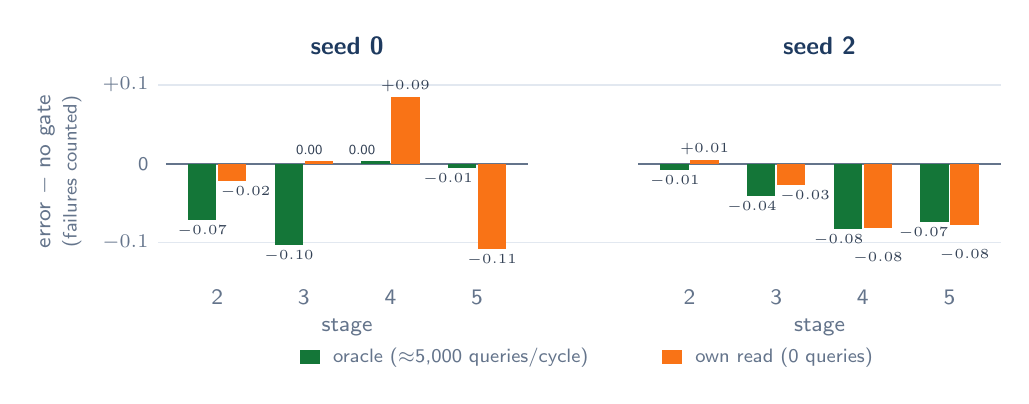
\begin{tikzpicture}[x=1cm,y=1cm]
  \def\ys{10}
  \foreach \t in {-0.1,0.1} {
    \draw[slate200, line width=0.5pt] (-0.1,\t*\ys) -- (10.6,\t*\ys);
    \node[note, font=\sffamily\scriptsize, anchor=east] at (-0.1,\t*\ys)
        {\pgfmathprintnumber[fixed,precision=1,showpos]{\t}};
  }
  \node[note, font=\sffamily\scriptsize, anchor=east] at (-0.1,0) {0};
  \node[note, rotate=90, anchor=south, align=center] at (-0.95,-0.1) {error $-$ no gate\\ \scriptsize (failures counted)};
  % bars from the shared macro; its value labels are silenced here (and the scope kept
  % out of the bounding box) and re-set below with local nudges so adjacent labels don't collide
  \begin{scope}[overlay]\renewcommand{\pgfmathprintnumber}[2][]{}\renewcommand{\sgnum}[1]{}%
  \dpanel{0}{}{-0.071,-0.103,0.004,-0.005}{-0.022,0.004,0.085,-0.108}{armoracle}{armread}
  \dpanel{6}{}{-0.008,-0.041,-0.083,-0.074}{0.005,-0.027,-0.082,-0.078}{armoracle}{armread}
  \end{scope}
  \foreach \x/\v/\dx/\dy in {0.46/-0.071/0/0, 0.84/-0.022/0.17/0, 1.56/-0.103/0/0, 1.94/0.004/-0.12/0,
                         2.66/0.004/-0.17/0, 3.04/0.085/0/0, 3.76/-0.005/-0.18/0, 4.14/-0.108/0/0,
                         6.46/-0.008/0/0, 6.84/0.005/0/0, 7.56/-0.041/-0.12/0, 7.94/-0.027/0.175/0,
                         8.66/-0.083/-0.12/0, 9.04/-0.082/0/-0.24, 9.76/-0.074/-0.14/0, 10.14/-0.078/0/-0.24} {
    \pgfmathsetmacro{\yl}{(\v>=0 ? \v*\ys+0.14 : \v*\ys-0.14)+\dy}
    \node[valnum] at (\x+\dx,\yl) {\sgnum{\v}};
  }
  \node[caphead, font=\sffamily\small\bfseries] at (2.3,1.5) {seed 0};
  \node[caphead, font=\sffamily\small\bfseries] at (8.3,1.5) {seed 2};
  \dstages{0}{-0.14}
  \dstages{6}{-0.14}
  \fill[armoracle] (1.7,-2.55) rectangle ++(0.25,0.18);
  \node[note, anchor=west, font=\sffamily\scriptsize] at (2.0,-2.46) {oracle ($\approx$5{,}000 queries/cycle)};
  \fill[armread] (6.3,-2.55) rectangle ++(0.25,0.18);
  \node[note, anchor=west, font=\sffamily\scriptsize] at (6.6,-2.46) {own read (0 queries)};
\end{tikzpicture}}
\end{center}
\end{frame}

% ── The read's cost is timing ─────────────────────────────────────────────────
\begin{frame}{The read must wait for experience one level up}
\begin{columns}[T]
\begin{column}{0.49\textwidth}
{\small To judge a chunk, the read evaluates its consumers one level up and needs \warmtext{512} of its own graded writes there. Level-3 chunks become usable only at cycle 100~/~77, so the read \textbf{lags by construction}: level-2 chunks are first judged at \textbf{105 / 80}, level-3 at 197, level-4 never. Meanwhile junk enters unchecked.}

\smallskip
\begin{alertblock}{Takeaway}
{\small No grader queries, but it costs time: blind habit keeps mistakes during the wait.}
\end{alertblock}
\end{column}

\begin{column}{0.49\textwidth}
\centering
\resizebox{\linewidth}{!}{%
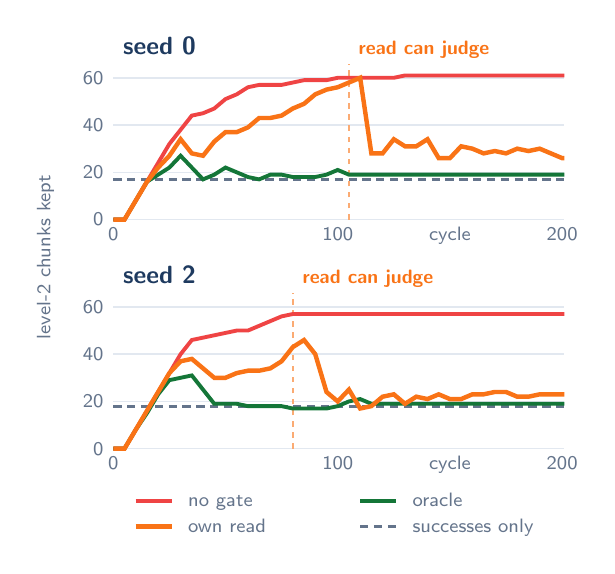
\begin{tikzpicture}[x=0.0285cm,y=0.030cm]
  \foreach \py/\ttl/\fl/\orc/\rd/\mk/\ref in {97/seed 0/\serAfloortot/\serAoracletot/\serAreadtot/105/17,
                                              0/seed 2/\serBfloortot/\serBoracletot/\serBreadtot/80/18} {
    \begin{scope}[shift={(0,\py)}]
      \foreach \t in {0,20,40,60} {
        \draw[slate200, line width=0.5pt] (0,\t) -- (201,\t);
        \node[note, font=\sffamily\scriptsize, anchor=east] at (0,\t) {\t};
      }
      \draw[armref, line width=1pt, dash pattern=on 3pt off 2pt] (0,\ref) -- (201,\ref);
      \draw[armread!60, line width=0.8pt, dash pattern=on 2pt off 2pt] (\mk,0) -- (\mk,66);
      \node[font=\sffamily\scriptsize\bfseries, text=armread, anchor=base west] at (\mk,70) {read can judge};
      \draw[armfloor, line width=1.4pt] \fl;
      \draw[armoracle, line width=1.4pt] \orc;
      \draw[armread, line width=1.6pt] \rd;
      \foreach \c in {0,100,200} {\node[note, font=\sffamily\scriptsize, anchor=base] at (\c,-9) {\c};}
      \node[note, font=\sffamily\scriptsize, anchor=base] at (150,-9) {cycle};
      \node[caphead, font=\sffamily\small\bfseries, anchor=base west] at (0,70) {\ttl};
    \end{scope}
  }
  \node[note, rotate=90, anchor=south, font=\sffamily\scriptsize] at (-22,81) {level-2 chunks kept};
  % legend
  \draw[armfloor, line width=1.4pt] (10,-22) -- ++(16,0); \node[note, anchor=base west, font=\sffamily\scriptsize] at (29,-24.5) {no gate};
  \draw[armoracle, line width=1.4pt] (110,-22) -- ++(16,0); \node[note, anchor=base west, font=\sffamily\scriptsize] at (129,-24.5) {oracle};
  \draw[armread, line width=1.6pt] (10,-33) -- ++(16,0); \node[note, anchor=base west, font=\sffamily\scriptsize] at (29,-35.5) {own read};
  \draw[armref, line width=1pt, dash pattern=on 3pt off 2pt] (110,-33) -- ++(16,0); \node[note, anchor=base west, font=\sffamily\scriptsize] at (129,-35.5) {successes only};
\end{tikzpicture}}
\end{column}
\end{columns}
\end{frame}

% ── Once it can judge ─────────────────────────────────────────────────────────
\begin{frame}{Once it can judge, the read catches about half of what the oracle catches}
\begin{columns}[T]
\begin{column}{0.44\textwidth}
{\small The read-gated runs also record the oracle's verdict, unused. Where the oracle would remove a level-2 chunk, the read removes it \textbf{42\%~/~45\%} of the time; where it would keep one, the read removes it \textbf{10\%~/~18\%}.}

\smallskip
{\small At a chunk's own level, with far more experience, the read ranks oracle-useful chunks above useless ones (AUC $\approx$ 0.75), but its zero point is off: most true chunks get negative gains too.}
\end{column}

\begin{column}{0.54\textwidth}
\centering
\resizebox{\linewidth}{!}{%
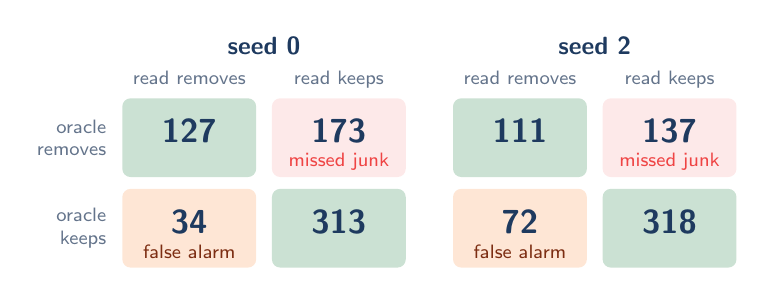
\begin{tikzpicture}[x=1cm,y=1cm]
  \foreach \px/\seed/\rr/\rk/\kr/\kk in {0/seed 0/127/173/34/313, 4.2/seed 2/111/137/72/318} {
    \begin{scope}[shift={(\px,0)}]
      \node[caphead, font=\sffamily\small\bfseries] at (2.2,2.82) {\seed};
      \node[note, font=\sffamily\scriptsize, anchor=base] at (1.25,2.32) {read removes};
      \node[note, font=\sffamily\scriptsize, anchor=base] at (3.15,2.32) {read keeps};
      \fill[armoracle!22, rounded corners=3pt] (0.4,1.15) rectangle ++(1.7,1.0);
      \fill[failc!12, rounded corners=3pt]     (2.3,1.15) rectangle ++(1.7,1.0);
      \fill[gateorange!18, rounded corners=3pt](0.4,0) rectangle ++(1.7,1.0);
      \fill[armoracle!22, rounded corners=3pt] (2.3,0) rectangle ++(1.7,1.0);
      \node[font=\sffamily\large\bfseries, text=maindark] at (1.25,1.73) {\rr};
      \node[font=\sffamily\large\bfseries, text=maindark] at (3.15,1.73) {\rk};
      \node[font=\sffamily\large\bfseries, text=maindark] at (1.25,0.58) {\kr};
      \node[font=\sffamily\large\bfseries, text=maindark] at (3.15,0.58) {\kk};
      \node[note, font=\sffamily\scriptsize, text=failc] at (3.15,1.35) {missed junk};
      \node[note, font=\sffamily\scriptsize, text=gatedark] at (1.25,0.2) {false alarm};
    \end{scope}
  }
  \node[note, font=\sffamily\scriptsize, anchor=east, align=right] at (0.32,1.65) {oracle\\removes};
  \node[note, font=\sffamily\scriptsize, anchor=east, align=right] at (0.32,0.5) {oracle\\keeps};
\end{tikzpicture}}

\dimtext{\scriptsize level-2 decisions, same tried problems}

\raggedright
\medskip
\begin{block}{Proposed next step}
{\small Judge at the chunk's own level first, with a calibrated threshold, then through its consumers.}
\end{block}
\end{column}
\end{columns}
\end{frame}

% ══════════════════════════════════════════════════════════════════════════════
\section{What it means}
% ══════════════════════════════════════════════════════════════════════════════

% ── What is not recovered ─────────────────────────────────────────────────────
\begin{frame}{Neither gate fully recovers last-stage performance}
\begin{columns}[T]
\begin{column}{0.5\textwidth}
{\small Both gates end \textbf{0.13--0.24} above the successes-only learner at the last stage, on both seeds. The data do not distinguish three possible causes:\par}

{\footnotesize
\begin{itemize}\itemsep2pt
  \item the top level is never judged, since nothing sits above it; its phrasebook stays two to three times the successes-only size;
  \item churn: about 270 removals and 150 re-offers per run, against 14 and 6 when only successes count;
  \item early practice used a polluted phrasebook.
\end{itemize}}

\smallskip
{\footnotesize These estimates rest on few cycles: the last two stages last 12 and 9 cycles, with one run per seed.\par}
\end{column}

\begin{column}{0.47\textwidth}
\centering
\resizebox{\linewidth}{!}{%
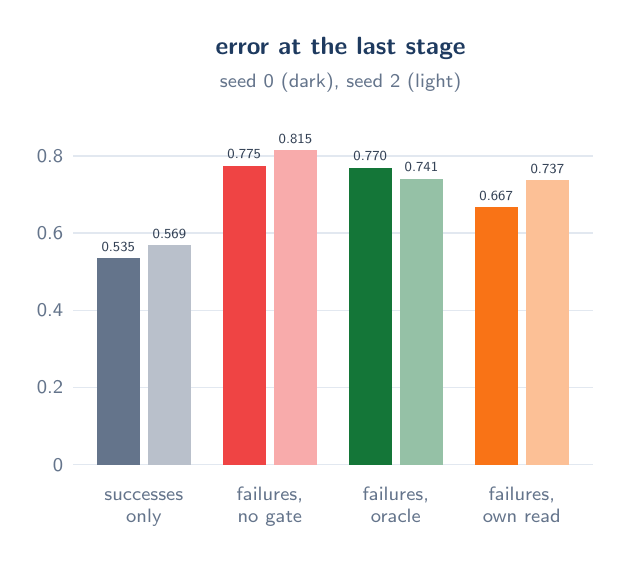
\begin{tikzpicture}[x=1cm,y=4.9cm]
  \foreach \t in {0,0.2,0.4,0.6,0.8} {
    \draw[slate200, line width=0.5pt] (-0.1,\t) -- (6.5,\t);
    \node[note, font=\sffamily\scriptsize, anchor=east] at (-0.1,\t) {\t};
  }
  \foreach \i/\c/\a/\b/\lab in {0/armref/0.535/0.569/{successes\\only},
                                 1/armfloor/0.775/0.815/{failures,\\no gate},
                                 2/armoracle/0.770/0.741/{failures,\\oracle},
                                 3/armread/0.667/0.737/{failures,\\own read}} {
    \pgfmathsetmacro{\xx}{\i*1.6+0.2}
    \fill[\c] (\xx,0) rectangle ++(0.55,\a);
    \fill[\c!45] (\xx+0.65,0) rectangle ++(0.55,\b);
    \node[valnum] at (\xx+0.275,\a+0.03) {\a};
    \node[valnum] at (\xx+0.925,\b+0.03) {\b};
    \node[note, font=\sffamily\scriptsize, anchor=base, align=center] at (\xx+0.6,-0.15) {\lab};
  }
  \node[caphead, font=\sffamily\small\bfseries] at (3.3,1.08) {error at the last stage};
  \node[note, font=\sffamily\scriptsize] at (3.3,0.99) {seed 0 (dark), seed 2 (light)};
\end{tikzpicture}}
\end{column}
\end{columns}
\end{frame}

% ── Synthesis ─────────────────────────────────────────────────────────────────
\begin{frame}{A value gate pays off when habit is blind to outcome}
\begin{center}
\resizebox{0.97\linewidth}{!}{%
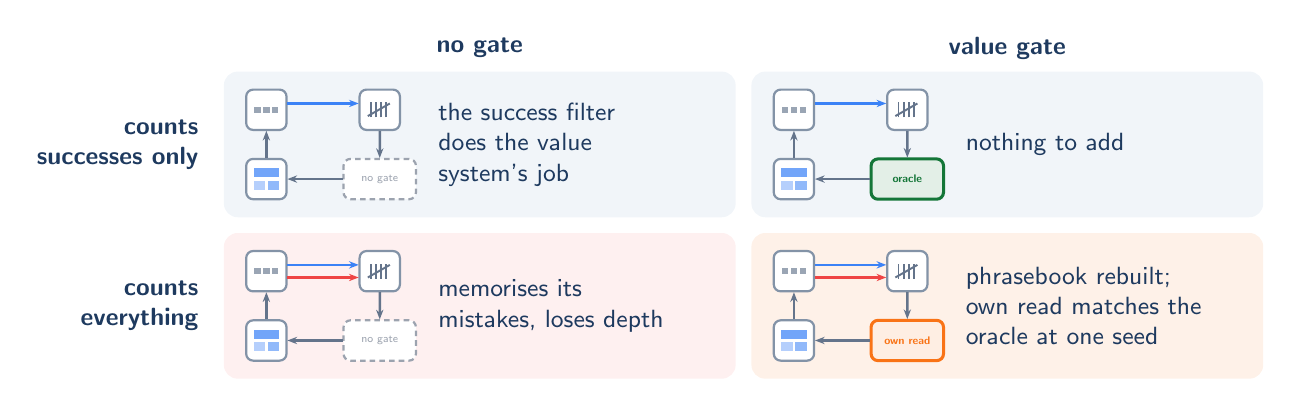
\begin{tikzpicture}[x=1cm,y=1cm]
  \node[caphead, font=\sffamily\small\bfseries] at (3.25,4.2) {no gate};
  \node[caphead, font=\sffamily\small\bfseries] at (9.95,4.2) {value gate};
  \node[caphead, font=\sffamily\small\bfseries, anchor=east, align=right] at (-0.2,2.975) {counts\\successes only};
  \node[caphead, font=\sffamily\small\bfseries, anchor=east, align=right] at (-0.2,0.925) {counts\\everything};
  % cells: 6.5 x 1.85, glyph (0.8x) centred vertically at the left, text anchored at a common x
  \foreach \x/\y/\fc/\f/\g/\txt [count=\ci] in {
      0/2.05/slate100/0/0/{the success filter\\does the value\\system's job},
      6.7/2.05/slate100/0/1/{nothing to add},
      0/0/failc!8/1/0/{memorises its\\mistakes, loses depth},
      6.7/0/gateorange!10/1/2/{phrasebook rebuilt;\\own read matches the\\oracle at one seed}} {
    \fill[\fc, rounded corners=5pt] (\x,\y) rectangle ++(6.5,1.85);
    \begin{scope}[shift={(\x+0.54,\y+0.485)}, scale=0.8, transform shape, name prefix=s\ci-]
      \loopglyph{\f}{\g}
    \end{scope}
    \node[font=\sffamily\small, text=maindark, anchor=west, align=left] at (\x+2.6,\y+0.925) {\txt};
  }
\end{tikzpicture}}
\end{center}

\smallskip
{\small Goal-directed behaviour in the wild looks like the bottom row: candidates are abundant, habits form by repetition, and the hard part is knowing which to keep. \textbf{Habit and value need each other}: \hltext{the habit loop's graded attempts train the read}, and \warmtext{the read decides what the habit loop keeps}.}
\end{frame}

% ── Summary ───────────────────────────────────────────────────────────────────
{
\setbeamercolor{background canvas}{bg=slate800}
\setbeamercolor{normal text}{fg=white}
\usebeamercolor[fg]{normal text}
\begin{frame}[plain,noframenumbering]
\vfill
\begin{center}
{\Large\bfseries\textcolor{white}{A value gate pays off when habit is blind to outcome}}\\[18pt]
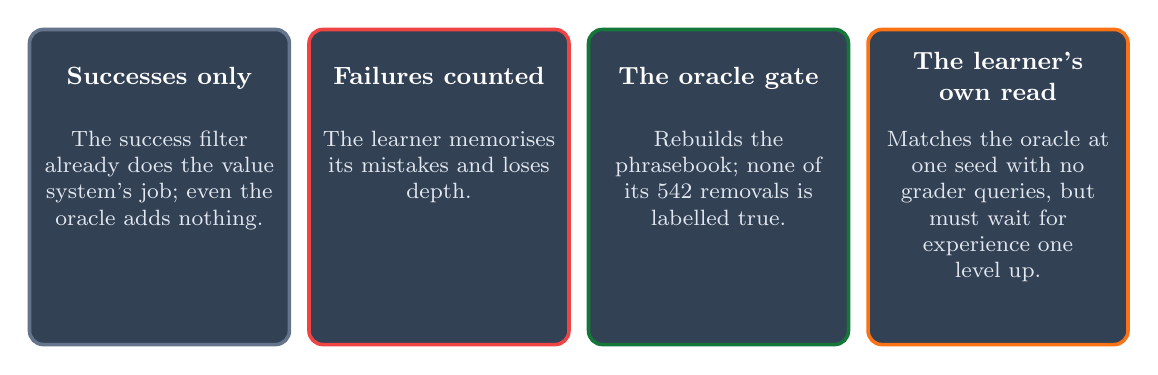
\begin{tikzpicture}[x=1cm,y=1cm]
  \foreach \i/\c/\h/\t in {
      0/armref/{Successes only}/{The success filter already does the value system's job; even the oracle adds nothing.},
      1/armfloor/{Failures counted}/{The learner memorises its mistakes and loses depth.},
      2/armoracle/{The oracle gate}/{Rebuilds the phrasebook; none of its 542 removals is labelled true.},
      3/armread/{The learner's own~read}/{Matches the oracle at one seed with no grader queries, but must wait for experience one level~up.}} {
    \node[draw=\c, line width=1.3pt, fill=slate700, rounded corners=5pt, inner sep=5pt,
          anchor=north] at (\i*3.55,0) {%
      \begin{minipage}[t][3.65cm][t]{2.95cm}\centering
        \parbox[c][0.9cm][c]{\linewidth}{\centering\small\bfseries\strut\textcolor{white}{\h}\strut\par}\par
        \vspace{5pt}
        {\footnotesize\textcolor{slate200}{\t}\par}
      \end{minipage}};
  }
\end{tikzpicture}
\end{center}
\vfill
\end{frame}
}

\end{document}
